\documentclass[border=8pt]{standalone}
\usepackage[T1]{fontenc}
\usepackage[utf8]{inputenc}
\usepackage{circuitikz}
\usepackage{amsmath,amssymb}
\usetikzlibrary{positioning,calc,backgrounds}
\ctikzset{bipoles/length=1.0cm, font=\small}

\definecolor{fondo}{HTML}{0B0F17}
\definecolor{tinta}{HTML}{E2E8F0}
\definecolor{ambar}{HTML}{FB923C}
\definecolor{cyan}{HTML}{38BDF8}
\definecolor{verde}{HTML}{4ADE80}
\definecolor{rojo}{HTML}{F87171}
\definecolor{gris}{HTML}{64748B}

\begin{document}
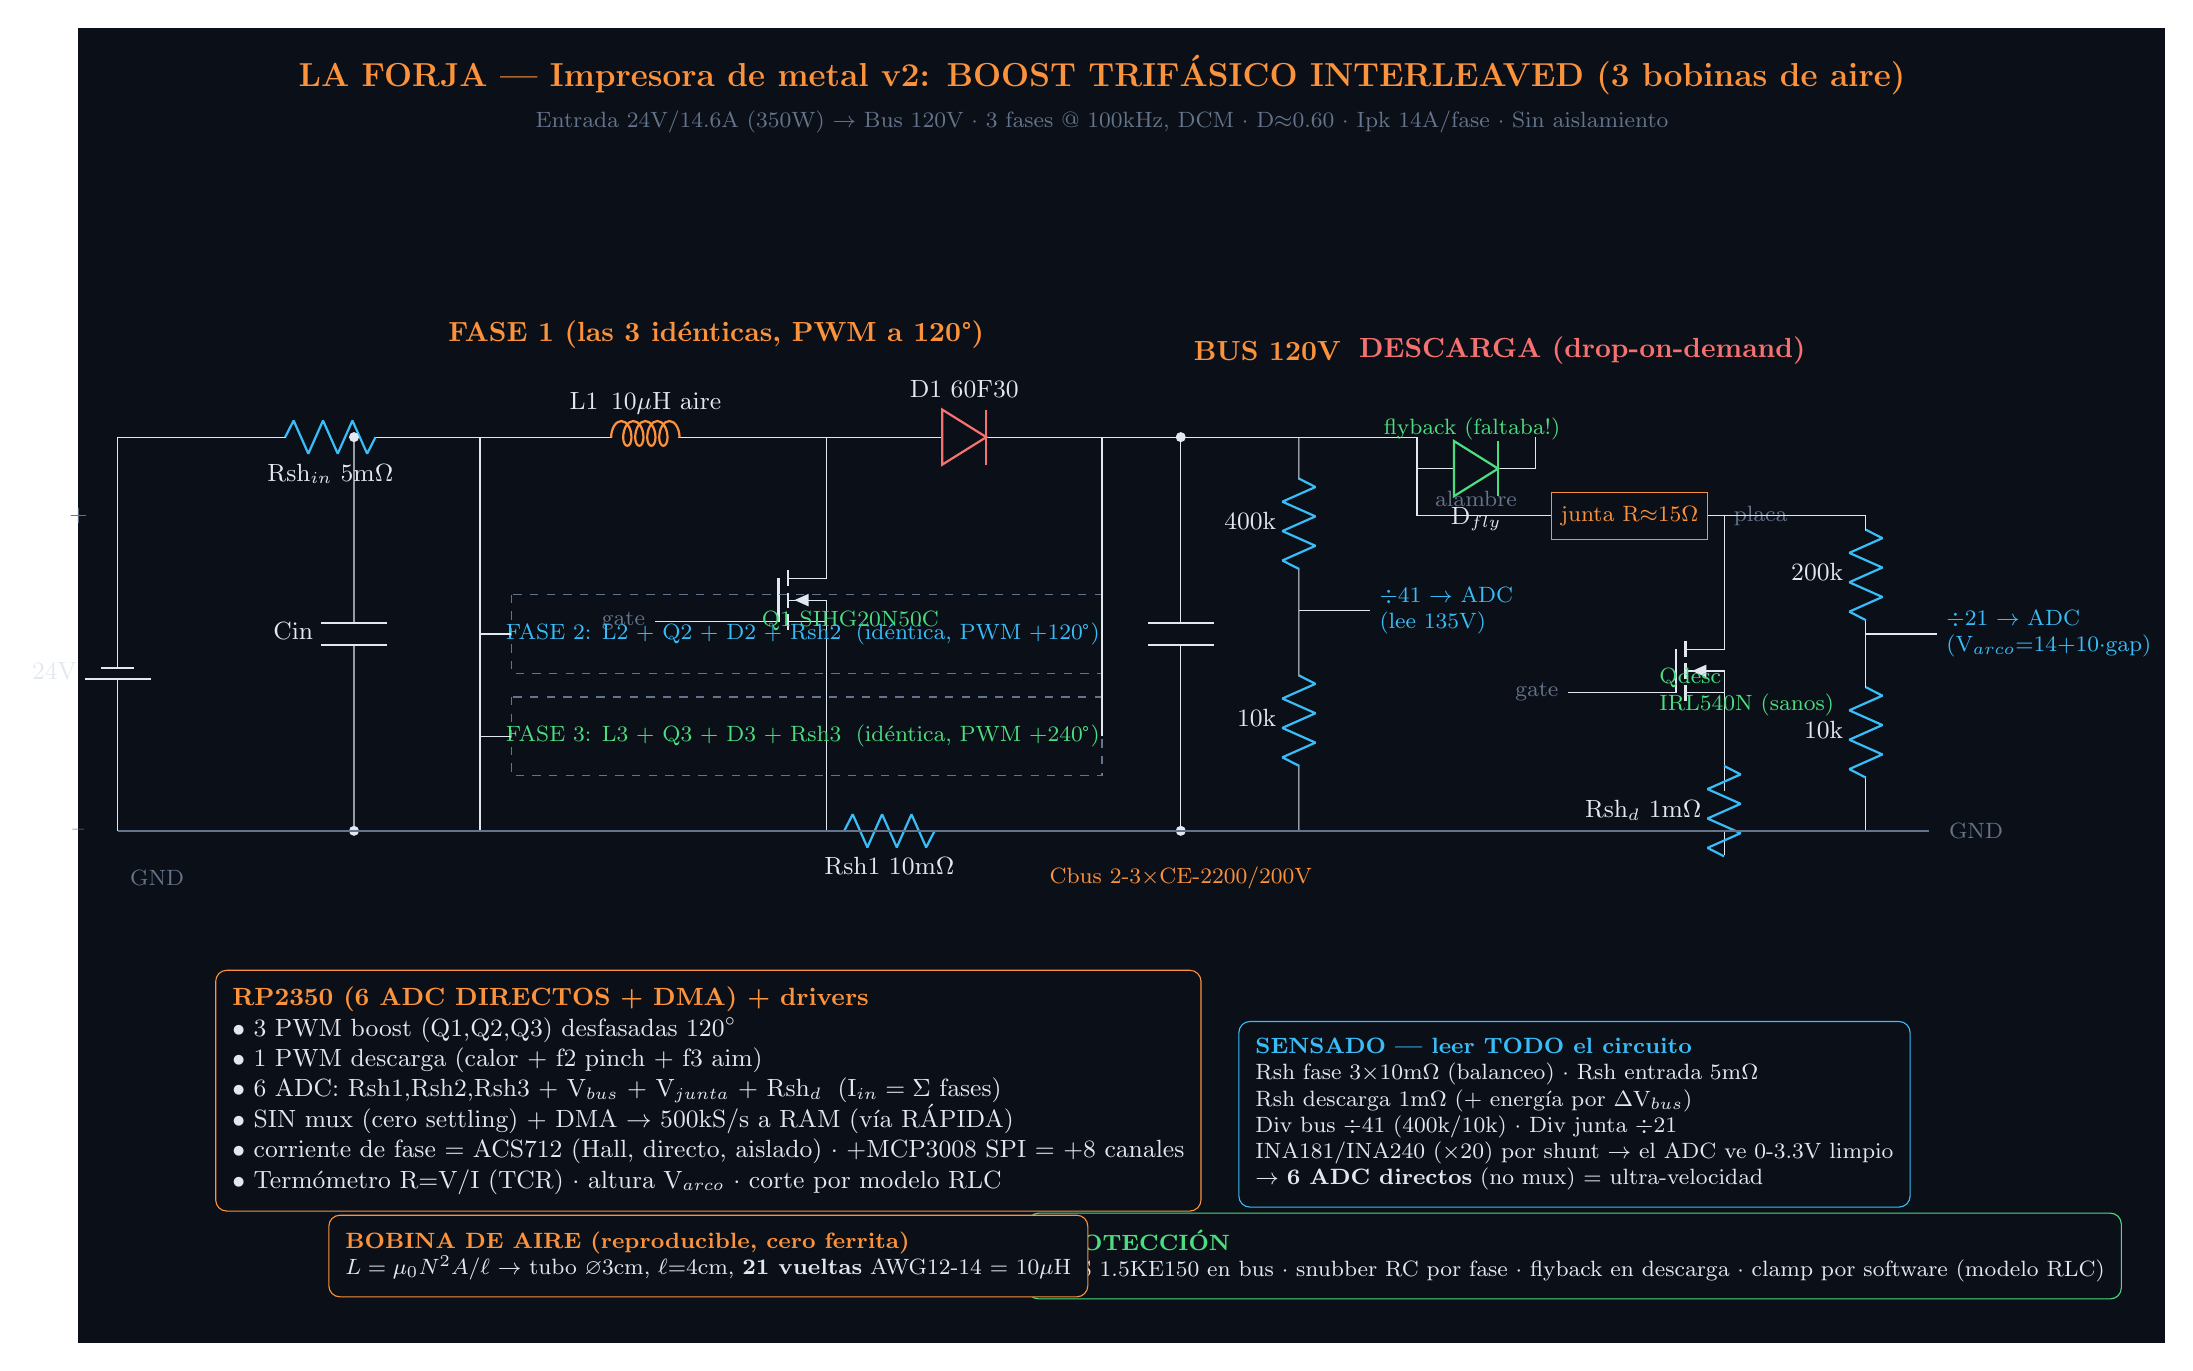
\begin{tikzpicture}[font=\small, every node/.style={text=tinta}]
\fill[fondo] (-2.5,-13.5) rectangle (24,3.2);

% ===================== TITULO =====================
\node[text=ambar, font=\bfseries\large] at (10.5,2.6) {LA FORJA — Impresora de metal v2: BOOST TRIFÁSICO INTERLEAVED (3 bobinas de aire)};
\node[text=gris, font=\footnotesize] at (10.5,2.0) {Entrada 24V/14.6A (350W) $\rightarrow$ Bus 120V $\cdot$ 3 fases @ 100kHz, DCM $\cdot$ D$\approx$0.60 $\cdot$ Ipk 14A/fase $\cdot$ Sin aislamiento};

\begin{scope}[color=tinta]

% ===================== ENTRADA 24V =====================
\draw (-2,-7) to[battery1, l=24V] (-2,-3);   % + arriba (al riel), - abajo (GND)
\node[text=gris,font=\footnotesize] at (-2.5,-3) {+}; \node[text=gris,font=\footnotesize] at (-2.5,-7) {--};
\draw (-2,-3) -- (-2,-2) -- (-0.3,-2);
\draw (-0.3,-2) to[R, l_={Rsh$_{in}$ 5m$\Omega$}, color=cyan] (1.7,-2);  % shunt entrada
\draw (1.7,-2) -- (2.6,-2);
\draw (1.0,-2) to[C, l_={Cin}, *-*] (1.0,-7);
\draw (2.6,-2) -- (2.6,-7);                      % riel + de entrada (a las 3 fases)
\draw (-2,-7) -- (2.6,-7);                        % GND entrada
\node[text=gris,font=\footnotesize,align=left] at (-1.5,-7.6) {GND};

% ===================== FASE 1 (detallada) =====================
\node[text=ambar,font=\bfseries] at (5.6,-0.7) {FASE 1 (las 3 idénticas, PWM a 120°)};
\draw (2.6,-2) -- (3.2,-2);
\draw (3.2,-2) to[L, l=L1 \,10$\mu$H aire, color=ambar] (6.2,-2);  % bobina de aire
\draw (6.2,-2) -- (7.0,-2) coordinate(sw1);                        % nodo SW
% MOSFET Q1 (low-side)
\draw (sw1) -- (7.0,-2);
\node[nigfete, anchor=D, rotate=0] (Q1) at (7.0,-3.3) {};
\draw (sw1) -- (Q1.D);
\draw (Q1.S) -- (7.0,-7);
\node[text=verde,font=\footnotesize,right=1pt of Q1.G] {Q1 SIHG20N50C};
\draw (Q1.G) -- ++(-1.2,0) node[left,text=gris,font=\footnotesize]{gate};
% shunt de fase
\draw (7.0,-7) to[R, l_={Rsh1 10m$\Omega$}, color=cyan] (8.6,-7);
% diodo D1 a bus
\draw (sw1) to[D, l=D1 60F30, color=rojo] (10.5,-2);

% ===================== FASES 2 y 3 (bloques) =====================
\draw[dashed,gris] (3.0,-4.0) rectangle (10.5,-5.0);
\node[text=cyan,font=\footnotesize] at (6.7,-4.5) {FASE 2: L2 + Q2 + D2 + Rsh2 \;(idéntica, PWM +120°)};
\draw[dashed,gris] (3.0,-5.3) rectangle (10.5,-6.3);
\node[text=verde,font=\footnotesize] at (6.7,-5.8) {FASE 3: L3 + Q3 + D3 + Rsh3 \;(idéntica, PWM +240°)};
\draw (2.6,-4.5) -- (3.0,-4.5);  \draw (2.6,-5.8) -- (3.0,-5.8);   % alimentación
\draw (10.5,-4.5) -- (10.5,-2);  \draw (10.5,-5.8) -- (10.5,-2);   % salida a bus
\draw (8.6,-7) -- (10.5,-7) -- (10.5,-7);                          % GND fases

% ===================== BUS 120V =====================
\draw (10.5,-2) -- (12.2,-2) coordinate(bus);
\node[text=ambar,font=\bfseries] at (12.6,-0.9) {BUS 120V};
\draw (11.5,-2) to[C, *-*] (11.5,-7);
\node[text=ambar,font=\footnotesize,align=center] at (11.5,-7.6) {Cbus 2-3$\times$CE-2200/200V};
% divisor del bus
\draw (12.2,-2) -- (13.0,-2);
\draw (13.0,-2) to[R, l_={400k}, color=cyan] (13.0,-4.2);
\draw (13.0,-4.2) to[R, l_={10k}, color=cyan] (13.0,-7) ;
\draw (13.0,-4.2) -- (13.9,-4.2) node[right,text=cyan,font=\footnotesize,align=left]{$\div$41 $\to$ ADC\\(lee 135V)};
\draw (10.5,-7) -- (13.0,-7);
\draw (13.0,-2) -- (13.0,-2);

% ===================== DESCARGA =====================
\draw (12.2,-2) -- (14.5,-2);
\node[text=rojo,font=\bfseries] at (16.6,-0.9) {DESCARGA (drop-on-demand)};
\draw (14.5,-2) -- (14.5,-3.0);
% flyback diode (lo que faltaba)
\draw (14.5,-2.4) to[D, l_={D$_{fly}$}, color=verde, mirror] (16.0,-2.4);
\draw (16.0,-2.4) -- (16.0,-2) -- (16.0,-2);
\node[text=verde,font=\footnotesize] at (15.2,-1.9) {flyback (faltaba!)};
% alambre + junta + placa
\draw (14.5,-3.0) -- (16.0,-3.0) node[midway,above,font=\footnotesize,text=gris]{alambre};
\node[draw=ambar,fill=fondo,text=ambar,font=\footnotesize,minimum height=6mm] (junta) at (17.2,-3.0) {junta R$\approx$15$\Omega$};
\draw (16.0,-3.0) -- (junta.west);
\draw (junta.east) -- (18.4,-3.0) node[right,font=\footnotesize,text=gris]{placa};
\draw (18.4,-3.0) -- (18.4,-4.2);
% MOSFET descarga (low-side, los del v1 sanos)
\node[nigfete, anchor=D] (Qd) at (18.4,-4.2) {};
\draw (18.4,-4.2) -- (Qd.D);
\draw (Qd.S) -- (18.4,-6.5);
\node[text=verde,font=\footnotesize,right=1pt of Qd.G,align=left] {Qdesc\\IRL540N (sanos)};
\draw (Qd.G) -- ++(-1.0,0) node[left,text=gris,font=\footnotesize]{gate};
% shunt descarga
\draw (18.4,-6.5) to[R, l_={Rsh$_d$ 1m$\Omega$}, color=cyan] (18.4,-7) ;
\draw (16.0,-7) -- (18.4,-7);
% divisor V_junta
\draw (18.4,-3.0) -- (20.2,-3.0);
\draw (20.2,-3.0) to[R, l_={200k}, color=cyan] (20.2,-4.5);
\draw (20.2,-4.5) to[R, l_={10k}, color=cyan] (20.2,-7);
\draw (20.2,-4.5) -- (21.1,-4.5) node[right,text=cyan,font=\footnotesize,align=left]{$\div$21 $\to$ ADC\\(V$_{arco}$=14+10$\cdot$gap)};
\draw (18.4,-7) -- (20.2,-7);

% ===================== GND comun =====================
\draw[gris,thick] (-2,-7) -- (21.0,-7);
\node[text=gris,font=\footnotesize] at (21.6,-7) {GND};

% ===================== CEREBRO + SENSADO =====================
\node[draw=ambar,fill=fondo,text=tinta,rounded corners,align=left,inner sep=6pt] (cpu) at (5.5,-10.3)
 {\textbf{\textcolor{ambar}{RP2350 (6 ADC DIRECTOS + DMA) + drivers}}\\
  $\bullet$ 3 PWM boost (Q1,Q2,Q3) desfasadas 120$^\circ$\\
  $\bullet$ 1 PWM descarga (calor + f2 pinch + f3 aim)\\
  $\bullet$ 6 ADC: Rsh1,Rsh2,Rsh3 + V$_{bus}$ + V$_{junta}$ + Rsh$_d$ \;(I$_{in}=\Sigma$ fases)\\
  $\bullet$ SIN mux (cero settling) + DMA $\to$ 500kS/s a RAM (vía RÁPIDA)\\
  $\bullet$ corriente de fase = ACS712 (Hall, directo, aislado) $\cdot$ +MCP3008 SPI = +8 canales\\
  $\bullet$ Termómetro R=V/I (TCR) $\cdot$ altura V$_{arco}$ $\cdot$ corte por modelo RLC};

\node[draw=cyan,fill=fondo,text=tinta,rounded corners,align=left,inner sep=6pt,font=\footnotesize] (sens) at (16.5,-10.6)
 {\textbf{\textcolor{cyan}{SENSADO — leer TODO el circuito}}\\
  Rsh fase 3$\times$10m$\Omega$ (balanceo) $\cdot$ Rsh entrada 5m$\Omega$\\
  Rsh descarga 1m$\Omega$ (+ energía por $\Delta$V$_{bus}$)\\
  Div bus $\div$41 (400k/10k) $\cdot$ Div junta $\div$21\\
  INA181/INA240 ($\times$20) por shunt $\to$ el ADC ve 0-3.3V limpio\\
  $\rightarrow$ \textbf{6 ADC directos} (no mux) $=$ ultra-velocidad};

\node[draw=verde,fill=fondo,text=tinta,rounded corners,align=left,inner sep=6pt,font=\footnotesize] (prot) at (16.5,-12.4)
 {\textbf{\textcolor{verde}{PROTECCIÓN}}\\
  TVS 1.5KE150 en bus $\cdot$ snubber RC por fase $\cdot$ flyback en descarga $\cdot$ clamp por software (modelo RLC)};

\node[draw=ambar,fill=fondo,text=tinta,rounded corners,align=left,inner sep=6pt,font=\footnotesize] (bob) at (5.5,-12.4)
 {\textbf{\textcolor{ambar}{BOBINA DE AIRE (reproducible, cero ferrita)}}\\
  $L=\mu_0 N^2 A/\ell$ $\rightarrow$ tubo $\varnothing$3cm, $\ell$=4cm, \textbf{21 vueltas} AWG12-14 $=$ 10$\mu$H};

\end{scope}
\end{tikzpicture}
\end{document}
